%csbd_acl

\documentclass[../../main/main.tex]{subfiles}




\begin{document}
\title{Certified Security by Design (CSBD) \& Access\-Control Logic (ACL)}

%%%%%%%%%%%%%%%%%%%%% Chapter CSBD ACL %%%%%%%%%%%%%%%
\chapter[Certified Security by Design (CSBD) \& Access-Control Logic (ACL)]{Certified Security by Design (CSBD)  \\ \& \\ Access-Control Logic (ACL)} \label{chp:csbdacl}


      %%%%%%%%%%%%%%%%%%% Section CSBD %%%%%%%%%%%%%%%%%%
\section{Certified Security by Design (CSBD)} \label{sec:csbd}

\subsection{The Principle of Complete Mediation}\label{ssec:pcompletemediation}

      %%%%%%%%%%%%%%%%%%% Section ACL %%%%%%%%%%%%%%%%%%%
\section{Access-Control Logic (ACL)} \label{sec:acl}
\glsreset{acl}
\subsection{Motivation for Using ACL}\label{ssec:motivattionacl}
\subsection{ACL: A Command and Control (C2) Calculus} \label{ssec:aclc2}
\subsection{Principals}\label{ssec:principals}
\subsection{Well-formed Formulas Formulas}\label{ssec:wff}
\subsection{Kripke Structure}\label{ssec:kripke}
\subsubsection{satisies}\label{sssec:satisfies}
\subsubsection{soundness}\label{sssec:soundness}

\subsection{Inference Rules}\label{ssec:inferencerules}
The inference rules for the \gls{acl} are shown in figure \ref{inferencerules}.  All the inference rules are sound.  Details of proofs of soundness can be found in the text book \underline{Access Control, Security, and Trust: A Logical Approach}\cite{ChinOlder}.

\begin{figure}[h]
\centering
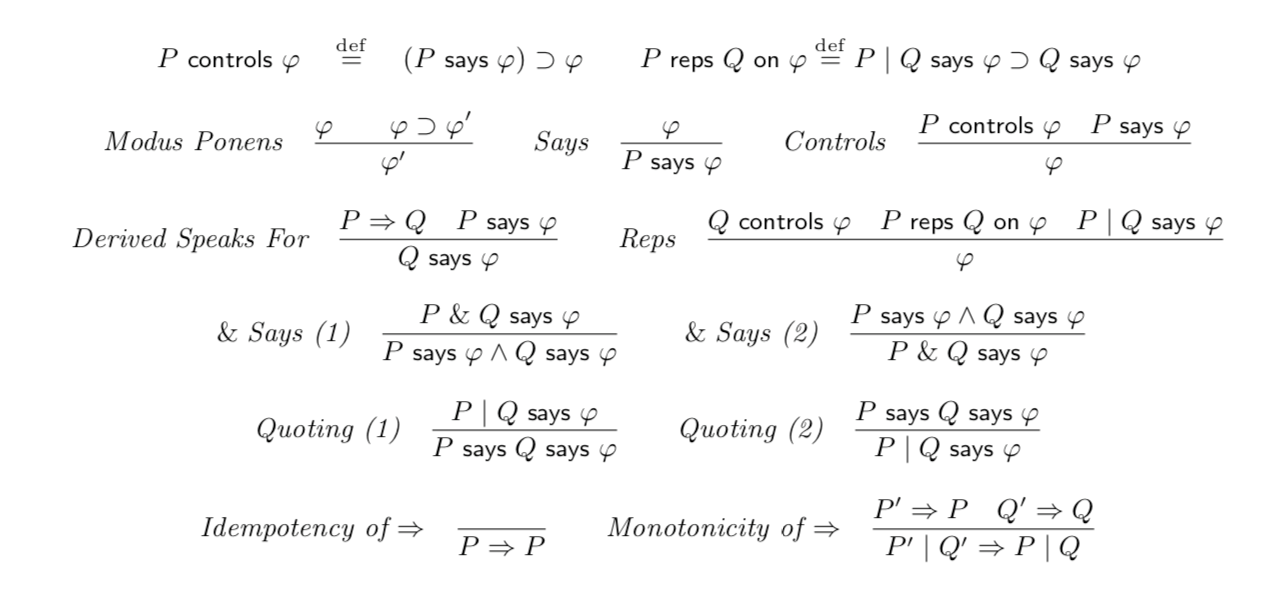
\includegraphics[width=\textwidth]{../figures/inferencerules}
\caption{\label{inferencerules}The \gls{acl} inference rules.}
\end{figure}

\subsection{Complete mediation}\label{ssec:aclcompletemediation}
Fundamental to this work is the concept of complete mediation (discussed in section \ref{ssec:pcompletemediation}).  In the \glsunset{acl}\gls{acl}, this means that each principal must be authenticated and authorized on each request.   ACL does this primarily by the \textit{Controls} inference rule in figure \ref{inferencerules} and shown again here in figure \ref{ControlsInferenceRule}. 

\begin{figure}[h]
\centering
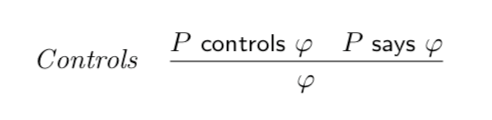
\includegraphics{../figures/ControlsInferenceRule}
\caption{\label{ControlsInferenceRule}The \textit{Controls} inference rule.}
\end{figure}

ACL refers to the left statement as an authorization \footnote{or a \textit{control} in the C2 calculus}.  The principal P controls (is authorized on) some action $\varphi$. ACL refers to the right statement in this inference rule as a request \footnote{or a \textit{command} in the C2 calculus}.  The principal P is requesting some action $\varphi$.The conjunction of the authorization and the request of P on $\varphi$ results in the action $\varphi$.  That is, if\textit{ P says $\varphi$} and \textit{P controls $\varphi$}  then $\varphi$  is true.  


\subsection{Well formed statements}
\subsection{Inference Rules}

      %%%%%%%%%%%%%%%%%%% Section ACL in HOL %%%%%%%%%%%%%%%
\section{ACL in HOL} \label{sec:aclinhol}
The equivalence of the \gls{acl} formulas implemented in HOL are shown in figure \ref{aclformulasHOL}.

\begin{figure}[h]
\centering
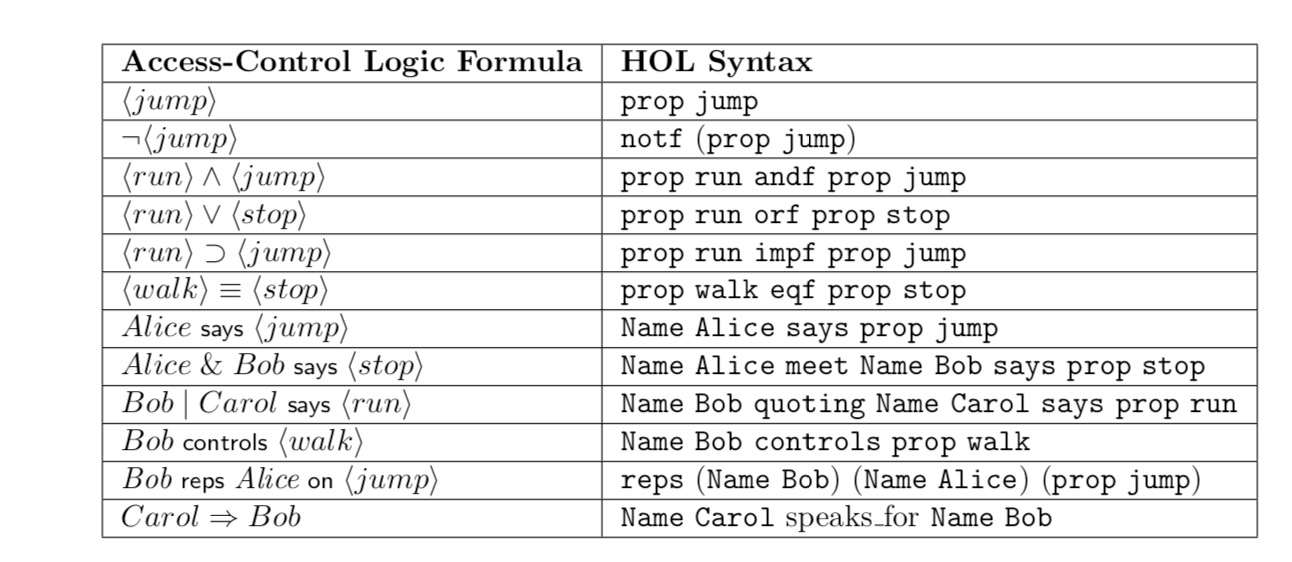
\includegraphics[width=\textwidth]{../figures/aclformulasHOL}
\caption{\label{aclformulasHOL}The \gls{acl} formulas in HOL.}
\end{figure}

Using this syntax, an ACL request of the form \textit{P says \textphi} would have the form
\centerline{ \textit{Name P says prop \textphi}}


\subsection{Complete Mediation}
\subsection{satList}



\end{document}

test acronym \glsentrytitlecase{acl}{desc}
more testing \glsentryname{acl}